% Options for packages loaded elsewhere
\PassOptionsToPackage{unicode}{hyperref}
\PassOptionsToPackage{hyphens}{url}
\PassOptionsToPackage{dvipsnames,svgnames,x11names}{xcolor}
%
\documentclass[
  letterpaper,
  DIV=11,
  numbers=noendperiod]{scrartcl}

\usepackage{amsmath,amssymb}
\usepackage{iftex}
\ifPDFTeX
  \usepackage[T1]{fontenc}
  \usepackage[utf8]{inputenc}
  \usepackage{textcomp} % provide euro and other symbols
\else % if luatex or xetex
  \usepackage{unicode-math}
  \defaultfontfeatures{Scale=MatchLowercase}
  \defaultfontfeatures[\rmfamily]{Ligatures=TeX,Scale=1}
\fi
\usepackage{lmodern}
\ifPDFTeX\else  
    % xetex/luatex font selection
\fi
% Use upquote if available, for straight quotes in verbatim environments
\IfFileExists{upquote.sty}{\usepackage{upquote}}{}
\IfFileExists{microtype.sty}{% use microtype if available
  \usepackage[]{microtype}
  \UseMicrotypeSet[protrusion]{basicmath} % disable protrusion for tt fonts
}{}
\makeatletter
\@ifundefined{KOMAClassName}{% if non-KOMA class
  \IfFileExists{parskip.sty}{%
    \usepackage{parskip}
  }{% else
    \setlength{\parindent}{0pt}
    \setlength{\parskip}{6pt plus 2pt minus 1pt}}
}{% if KOMA class
  \KOMAoptions{parskip=half}}
\makeatother
\usepackage{xcolor}
\setlength{\emergencystretch}{3em} % prevent overfull lines
\setcounter{secnumdepth}{-\maxdimen} % remove section numbering
% Make \paragraph and \subparagraph free-standing
\ifx\paragraph\undefined\else
  \let\oldparagraph\paragraph
  \renewcommand{\paragraph}[1]{\oldparagraph{#1}\mbox{}}
\fi
\ifx\subparagraph\undefined\else
  \let\oldsubparagraph\subparagraph
  \renewcommand{\subparagraph}[1]{\oldsubparagraph{#1}\mbox{}}
\fi


\providecommand{\tightlist}{%
  \setlength{\itemsep}{0pt}\setlength{\parskip}{0pt}}\usepackage{longtable,booktabs,array}
\usepackage{calc} % for calculating minipage widths
% Correct order of tables after \paragraph or \subparagraph
\usepackage{etoolbox}
\makeatletter
\patchcmd\longtable{\par}{\if@noskipsec\mbox{}\fi\par}{}{}
\makeatother
% Allow footnotes in longtable head/foot
\IfFileExists{footnotehyper.sty}{\usepackage{footnotehyper}}{\usepackage{footnote}}
\makesavenoteenv{longtable}
\usepackage{graphicx}
\makeatletter
\def\maxwidth{\ifdim\Gin@nat@width>\linewidth\linewidth\else\Gin@nat@width\fi}
\def\maxheight{\ifdim\Gin@nat@height>\textheight\textheight\else\Gin@nat@height\fi}
\makeatother
% Scale images if necessary, so that they will not overflow the page
% margins by default, and it is still possible to overwrite the defaults
% using explicit options in \includegraphics[width, height, ...]{}
\setkeys{Gin}{width=\maxwidth,height=\maxheight,keepaspectratio}
% Set default figure placement to htbp
\makeatletter
\def\fps@figure{htbp}
\makeatother

\usepackage{booktabs}
\usepackage{longtable}
\usepackage{array}
\usepackage{multirow}
\usepackage{wrapfig}
\usepackage{float}
\usepackage{colortbl}
\usepackage{pdflscape}
\usepackage{tabu}
\usepackage{threeparttable}
\usepackage{threeparttablex}
\usepackage[normalem]{ulem}
\usepackage{makecell}
\usepackage{xcolor}
\KOMAoption{captions}{tableheading}
\makeatletter
\@ifpackageloaded{caption}{}{\usepackage{caption}}
\AtBeginDocument{%
\ifdefined\contentsname
  \renewcommand*\contentsname{Table of contents}
\else
  \newcommand\contentsname{Table of contents}
\fi
\ifdefined\listfigurename
  \renewcommand*\listfigurename{List of Figures}
\else
  \newcommand\listfigurename{List of Figures}
\fi
\ifdefined\listtablename
  \renewcommand*\listtablename{List of Tables}
\else
  \newcommand\listtablename{List of Tables}
\fi
\ifdefined\figurename
  \renewcommand*\figurename{Figure}
\else
  \newcommand\figurename{Figure}
\fi
\ifdefined\tablename
  \renewcommand*\tablename{Table}
\else
  \newcommand\tablename{Table}
\fi
}
\@ifpackageloaded{float}{}{\usepackage{float}}
\floatstyle{ruled}
\@ifundefined{c@chapter}{\newfloat{codelisting}{h}{lop}}{\newfloat{codelisting}{h}{lop}[chapter]}
\floatname{codelisting}{Listing}
\newcommand*\listoflistings{\listof{codelisting}{List of Listings}}
\makeatother
\makeatletter
\makeatother
\makeatletter
\@ifpackageloaded{caption}{}{\usepackage{caption}}
\@ifpackageloaded{subcaption}{}{\usepackage{subcaption}}
\makeatother
\ifLuaTeX
  \usepackage{selnolig}  % disable illegal ligatures
\fi
\usepackage{bookmark}

\IfFileExists{xurl.sty}{\usepackage{xurl}}{} % add URL line breaks if available
\urlstyle{same} % disable monospaced font for URLs
\hypersetup{
  pdftitle={Environmental impact of utilities},
  colorlinks=true,
  linkcolor={blue},
  filecolor={Maroon},
  citecolor={Blue},
  urlcolor={Blue},
  pdfcreator={LaTeX via pandoc}}

\title{Environmental impact of utilities}
\author{Stan Brouwer}
\date{}

\begin{document}
\maketitle

With the recent focus on sustainability and net-zero by 2024, important
business decisions have to be made. To make these decisions, we need to
know our current environmental impact. This report models the
enivronmental impact of utilities, assuming gas, power and solar. The
numbers are based on typical residential building, but numbers for an
office can easily be plugged in.

\subsection{Utility consumption}\label{utility-consumption}

Assuming the following usage pattern:

\phantomsection\label{cell-fig-utility}
\begin{figure}[H]

\centering{

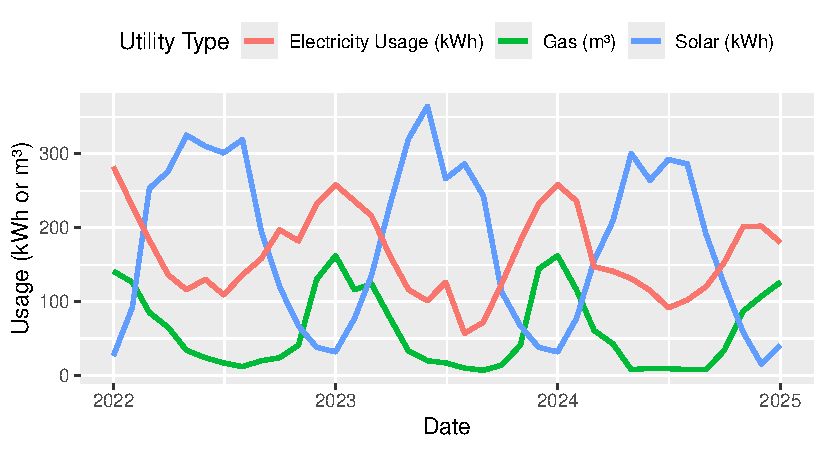
\includegraphics{index_files/figure-pdf/fig-utility-1.pdf}

}

\caption{\label{fig-utility}Assumed utility usage. Note that energy
meters measure net flow, and thus gross solar and power might differ.}

\end{figure}%

Details

\phantomsection\label{tbl-utility}
\begin{longtable}[]{@{}lrrr@{}}
\toprule\noalign{}
Date & Gas (m³) & Electricity Usage (kWh) & Solar (kWh) \\
\midrule\noalign{}
\endhead
\bottomrule\noalign{}
\endlastfoot
2025-01-01 & 126.0 & 180.0 & 40.6 \\
2024-12-01 & 107.0 & 202.0 & 15.4 \\
2024-11-01 & 86.9 & 201.0 & 58.4 \\
2024-10-01 & 33.8 & 153.0 & 123.0 \\
2024-09-01 & 8.2 & 120.0 & 191.0 \\
2024-08-01 & 8.1 & 102.0 & 286.0 \\
2024-07-01 & 9.2 & 91.5 & 292.0 \\
2024-06-01 & 9.7 & 115.0 & 264.0 \\
2024-05-01 & 7.9 & 131.0 & 300.0 \\
2024-04-01 & 42.8 & 141.0 & 209.0 \\
2024-03-01 & 60.9 & 147.0 & 155.0 \\
2024-02-01 & 116.0 & 236.0 & 77.0 \\
2024-01-01 & 162.0 & 258.0 & 32.0 \\
2023-12-01 & 144.0 & 232.0 & 38.0 \\
2023-11-01 & 41.0 & 182.0 & 67.0 \\
2023-10-01 & 14.0 & 124.0 & 113.0 \\
2023-09-01 & 7.0 & 72.0 & 243.0 \\
2023-08-01 & 10.0 & 57.0 & 286.0 \\
2023-07-01 & 17.0 & 126.0 & 266.0 \\
2023-06-01 & 20.0 & 101.0 & 364.0 \\
2023-05-01 & 33.0 & 116.0 & 320.0 \\
2023-04-01 & 77.0 & 161.0 & 232.0 \\
2023-03-01 & 124.0 & 216.0 & 135.0 \\
2023-02-01 & 116.0 & 236.0 & 77.0 \\
2023-01-01 & 162.0 & 258.0 & 32.0 \\
2022-12-01 & 130.0 & 232.0 & 38.0 \\
2022-11-01 & 41.0 & 182.0 & 67.0 \\
2022-10-01 & 24.0 & 197.0 & 120.0 \\
2022-09-01 & 20.0 & 158.0 & 195.0 \\
2022-08-01 & 12.0 & 136.0 & 319.0 \\
2022-07-01 & 17.0 & 109.0 & 301.0 \\
2022-06-01 & 24.0 & 130.0 & 310.0 \\
2022-05-01 & 34.0 & 116.0 & 325.0 \\
2022-04-01 & 65.0 & 136.0 & 276.0 \\
2022-03-01 & 85.0 & 183.0 & 253.0 \\
2022-02-01 & 126.0 & 229.0 & 92.0 \\
2022-01-01 & 141.0 & 282.0 & 27.0 \\
\end{longtable}

\subsection{Emissions of energy
production}\label{emissions-of-energy-production}

To quantify and compare the warming effects of different kind of
emissions, the IPPC proposes using the
\href{https://archive.ipcc.ch/ipccreports/tar/wg1/247.htm\#:~:text=The\%20GWP\%20has\%20been\%20defined,reference\%20gas\%20(IPCC\%2C\%20l990)\%3A}{Global
Warming Potential} (GWP), which can be used to express the warming
effect of different emissions to that of CO₂. To calculate our total
emissions, we must first determine the emissions caused by the energy
production.

\subsubsection{Electricity}\label{electricity}

The emissions of electricity production depends on the source of the
energy, which changes minute-by-minute. During day, a lot of green solar
power is generated, and during peaks, gas turbines kick in. Exact
information on the current national energy mix is
\href{https://ned.nl/nl/dataportaal/energie-productie/elektriciteit/totale-elektriciteitsproductie}{publicly
available}.
\href{https://ember-energy.org/data/electricity-data-explorer/\#data-tool}{Ember-energy}
calculates the CO₂ emissions based on the energy mix, and has an API
(email required) which provides the following numbers:

See also:
https://www.cbs.nl/-/media/\_excel/2023/06/1-co2-emissie-energieverbruik-rendementen-elektriciteit-2021.xls

\phantomsection\label{cell-fig-energy-intensity}
\begin{figure}[H]

\centering{

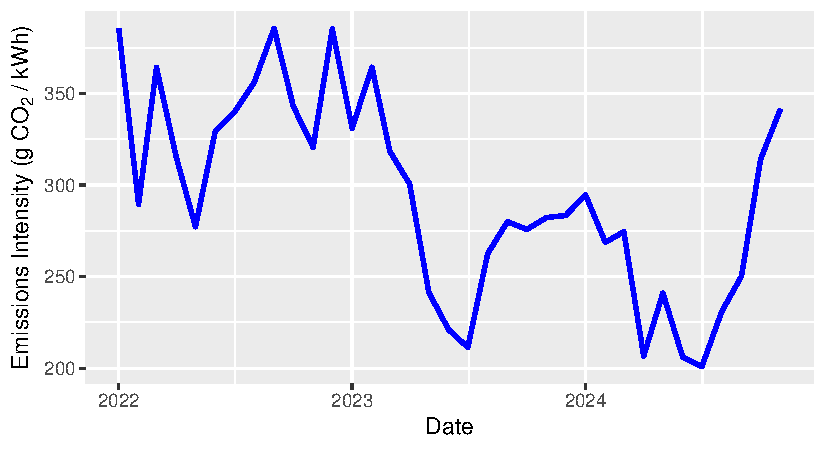
\includegraphics{index_files/figure-pdf/fig-energy-intensity-1.pdf}

}

\caption{\label{fig-energy-intensity}CO₂ emissions of the dutch energy
production over time}

\end{figure}%

To calculate the emissions caused by our energy consumption, we should
account for the differing CO₂ emissions as follows:

\[
\text{CO}_2  = \sum_{i=1}^{n} E_i \times F_i 
\] With \(\text{CO}_2\) is the total produced CO₂ in grams,\\
\(E_i\) the electricity usage for month \(i\) in kWh,\\
\(F_i\) the emissions intensity in \(g CO₂/kWh\) for that specific month
\(i\).

\subsubsection{Gas}\label{gas}

Calculating the exact emissions caused by gas production is somewhat
more complex as gas distributors measure the gas-usage as volume (m³)
which is dependent on the temperature, pressure and
\href{https://eduweb.eeni.tbm.tudelft.nl/TB141E/?aardgas-conversie}{gas
mix}, all of which are subject to change. Gas distributors solve this by
multiply the measured volume with a correction value to determine the
caloric value of the consumed gas (also see
\href{https://eduweb.eeni.tbm.tudelft.nl/TB141E/?aardgas-conversie}{wobbe
index}). These corrections can be found on the final invoice.

The Netherlands Enterprise Agency (RVO) has calculated the
\href{https://www.rvo.nl/sites/default/files/2023-10/CO2-emissiefactor-aardgas-Nederlandse-rapportage-en-ETS-\%202023.pdf}{emission
factor} for natural gas to be \textbf{56.34 kg CO₂ per GJ} of energy.
This only includes the emissions caused by burning the gas, not from
producing it. The exact number differs by ±2\% per year due to
differences in the national gas mix, for instance through higher LNG
imports.

The CBS
\href{https://www.cbs.nl/nl-nl/onze-diensten/methoden/begrippen/joule}{reports}
that \textbf{1 GJ of natural gas corresponds to 31.6 m³}, thus we can
calculate the emissions per m³ as follows:

\[
\frac{56.34 \text{ kg}}{\text{GJ}}
\]

Since

\[
1 \text{ GJ} = 31.6 \text{ m}^3
\] we can compute:

\[
\frac{56.34}{31.6} \text{ kg/m}^3
\]

which simplifies to:

\[
1.78 \text{ kg CO}_2 \text{ per m}^3
\]

As the deviations for the emissions of the gas mix are
\textasciitilde2\%, we simplify the calculation by not accounting for
them.

\subsection{Calculations}\label{calculations}

From the emission factors per energy type the final formula can be
determined:

\[
\text{CO}_2 = \left( \sum_{i=1}^{n} E_i \times F_i \right) + \left( G \times 1,78 \right)
\] With \(\text{CO}_2\) as the total produced CO₂ in grams,\\
\(E_i\) the electricity usage for month \(i\) in kWh,\\
\(F_i\) the emissions intensity in \(kg CO₂/kWh\) for that specific
month \(i\). \(G\) the total gas usage in m³

Plugging our usage data into this formula gives us the following
emissions:

\phantomsection\label{cell-fig-emissions}
\begin{figure}[H]

\centering{

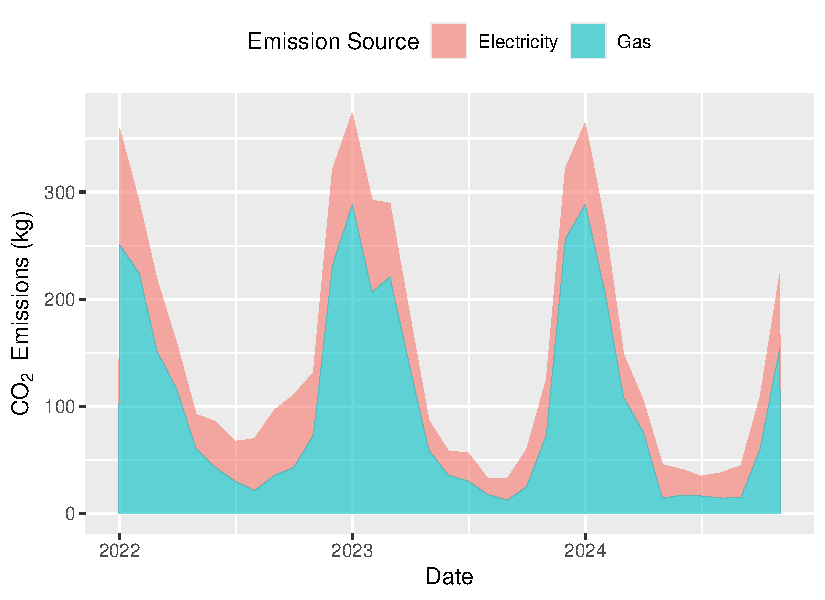
\includegraphics{index_files/figure-pdf/fig-emissions-1.pdf}

}

\caption{\label{fig-emissions}Monthly CO₂ Emissions from Energy and Gas}

\end{figure}%

\begin{longtable}[]{@{}cccc@{}}
\toprule\noalign{}
year & Gas emissions (kg CO₂) & Electricity emissions (kg CO₂) & Total
emissions (kg CO₂) \\
\midrule\noalign{}
\endhead
\bottomrule\noalign{}
\endlastfoot
2022 & 1279.82 & 721.12 & 2000.94 \\
2023 & 1361.70 & 551.89 & 1913.59 \\
2024 & 970.99 & 452.84 & 1423.83 \\
\end{longtable}

Details

\phantomsection\label{tbl-emissions}
\begin{longtable}[]{@{}lrrrl@{}}
\toprule\noalign{}
date & Electricity & Gas & total & year \\
\midrule\noalign{}
\endhead
\bottomrule\noalign{}
\endlastfoot
2024-11-01 & 68.62542 & 154.682 & 223.30742 & 2024 \\
2024-10-01 & 48.07719 & 60.164 & 108.24119 & 2024 \\
2024-09-01 & 30.03240 & 14.596 & 44.62840 & 2024 \\
2024-08-01 & 23.54670 & 14.418 & 37.96470 & 2024 \\
2024-07-01 & 18.37869 & 16.376 & 34.75469 & 2024 \\
2024-06-01 & 23.69920 & 17.266 & 40.96520 & 2024 \\
2024-05-01 & 31.56969 & 14.062 & 45.63169 & 2024 \\
2024-04-01 & 29.12778 & 76.184 & 105.31178 & 2024 \\
2024-03-01 & 40.34709 & 108.402 & 148.74909 & 2024 \\
2024-02-01 & 63.42028 & 206.480 & 269.90028 & 2024 \\
2024-01-01 & 76.01712 & 288.360 & 364.37712 & 2024 \\
2023-12-01 & 65.73720 & 256.320 & 322.05720 & 2023 \\
2023-11-01 & 51.36404 & 72.980 & 124.34404 & 2023 \\
2023-10-01 & 34.19300 & 24.920 & 59.11300 & 2023 \\
2023-09-01 & 20.16000 & 12.460 & 32.62000 & 2023 \\
2023-08-01 & 14.96307 & 17.800 & 32.76307 & 2023 \\
2023-07-01 & 26.62884 & 30.260 & 56.88884 & 2023 \\
2023-06-01 & 22.32100 & 35.600 & 57.92100 & 2023 \\
2023-05-01 & 27.99544 & 58.740 & 86.73544 & 2023 \\
2023-04-01 & 48.38694 & 137.060 & 185.44694 & 2023 \\
2023-03-01 & 68.77440 & 220.720 & 289.49440 & 2023 \\
2023-02-01 & 85.97480 & 206.480 & 292.45480 & 2023 \\
2023-01-01 & 85.39542 & 288.360 & 373.75542 & 2023 \\
2022-12-01 & 89.38264 & 231.400 & 320.78264 & 2022 \\
2022-11-01 & 58.34738 & 72.980 & 131.32738 & 2022 \\
2022-10-01 & 67.56115 & 42.720 & 110.28115 & 2022 \\
2022-09-01 & 60.91374 & 35.600 & 96.51374 & 2022 \\
2022-08-01 & 48.43504 & 21.360 & 69.79504 & 2022 \\
2022-07-01 & 37.03166 & 30.260 & 67.29166 & 2022 \\
2022-06-01 & 42.82070 & 42.720 & 85.54070 & 2022 \\
2022-05-01 & 32.15056 & 60.520 & 92.67056 & 2022 \\
2022-04-01 & 42.86040 & 115.700 & 158.56040 & 2022 \\
2022-03-01 & 66.65775 & 151.300 & 217.95775 & 2022 \\
2022-02-01 & 66.27718 & 224.280 & 290.55718 & 2022 \\
2022-01-01 & 108.68562 & 250.980 & 359.66562 & 2022 \\
\end{longtable}

If real estate occupancy rate, area or any other measure is known,
calculating the carbon footprint per person, workspace or area is
trivial.

\subsection{Concerns}\label{concerns}

Clearly, the current calculations only accounts for the direct emissions
caused by burning gas, or from producing electricity. (scope 1\&2
emissions). Producing and transporting gas and electricity also has a
significant impact on the environment.

Furthermore, solar panels return electricity into the grid. How should
they be accounted for?



\end{document}
